% Generated by final_parameter_analysis.py.
% This experiment evaluates a separable 1-D Taylor model applied independently along x and y. It is not the joint full 2-D Taylor model.
% separable 1-D Taylor along x/y; matched-clean metrics measure noise stability, not absolute derivative accuracy.
% Requires graphicx and booktabs.
\subsection{Parameter sensitivity and sparse joint selection}
\label{sec:final-parameter-analysis}
\graphicspath{{results/final_parameter_analysis/}{./}}

\paragraph{Scope and metric interpretation.}
This experiment evaluates a separable 1-D Taylor model applied independently along $x$ and $y$. It is not the joint full 2-D Taylor model. The matched-clean gradient RMSE and HOG metrics measure stability to injected noise for seed 42; they do not measure absolute derivative accuracy. All comparisons use parameter-matched clean references.
\emph{Model note: separable 1-D Taylor along $x/y$; matched-clean metrics measure noise stability, not absolute derivative accuracy.}

\paragraph{One-factor sensitivity.}
At fixed $h=1$, changing the per-axis sample count from $n=16$ to $n=32$ reduced correntropy gradient RMSE by 60.3\% under SP 5\% and 65.3\% under SP 10\%. The corresponding runtime changes were 54.2\% and 42.1\%, respectively. At fixed $n=8$, changing $h$ from 3 to 4 reduced correntropy RMSE by 21.6\% and 24.0\%, while the cosine gains were only 0.0049 and 0.0052. These statements apply only to the measured one-factor sweeps.

\begin{figure*}[t]
\centering
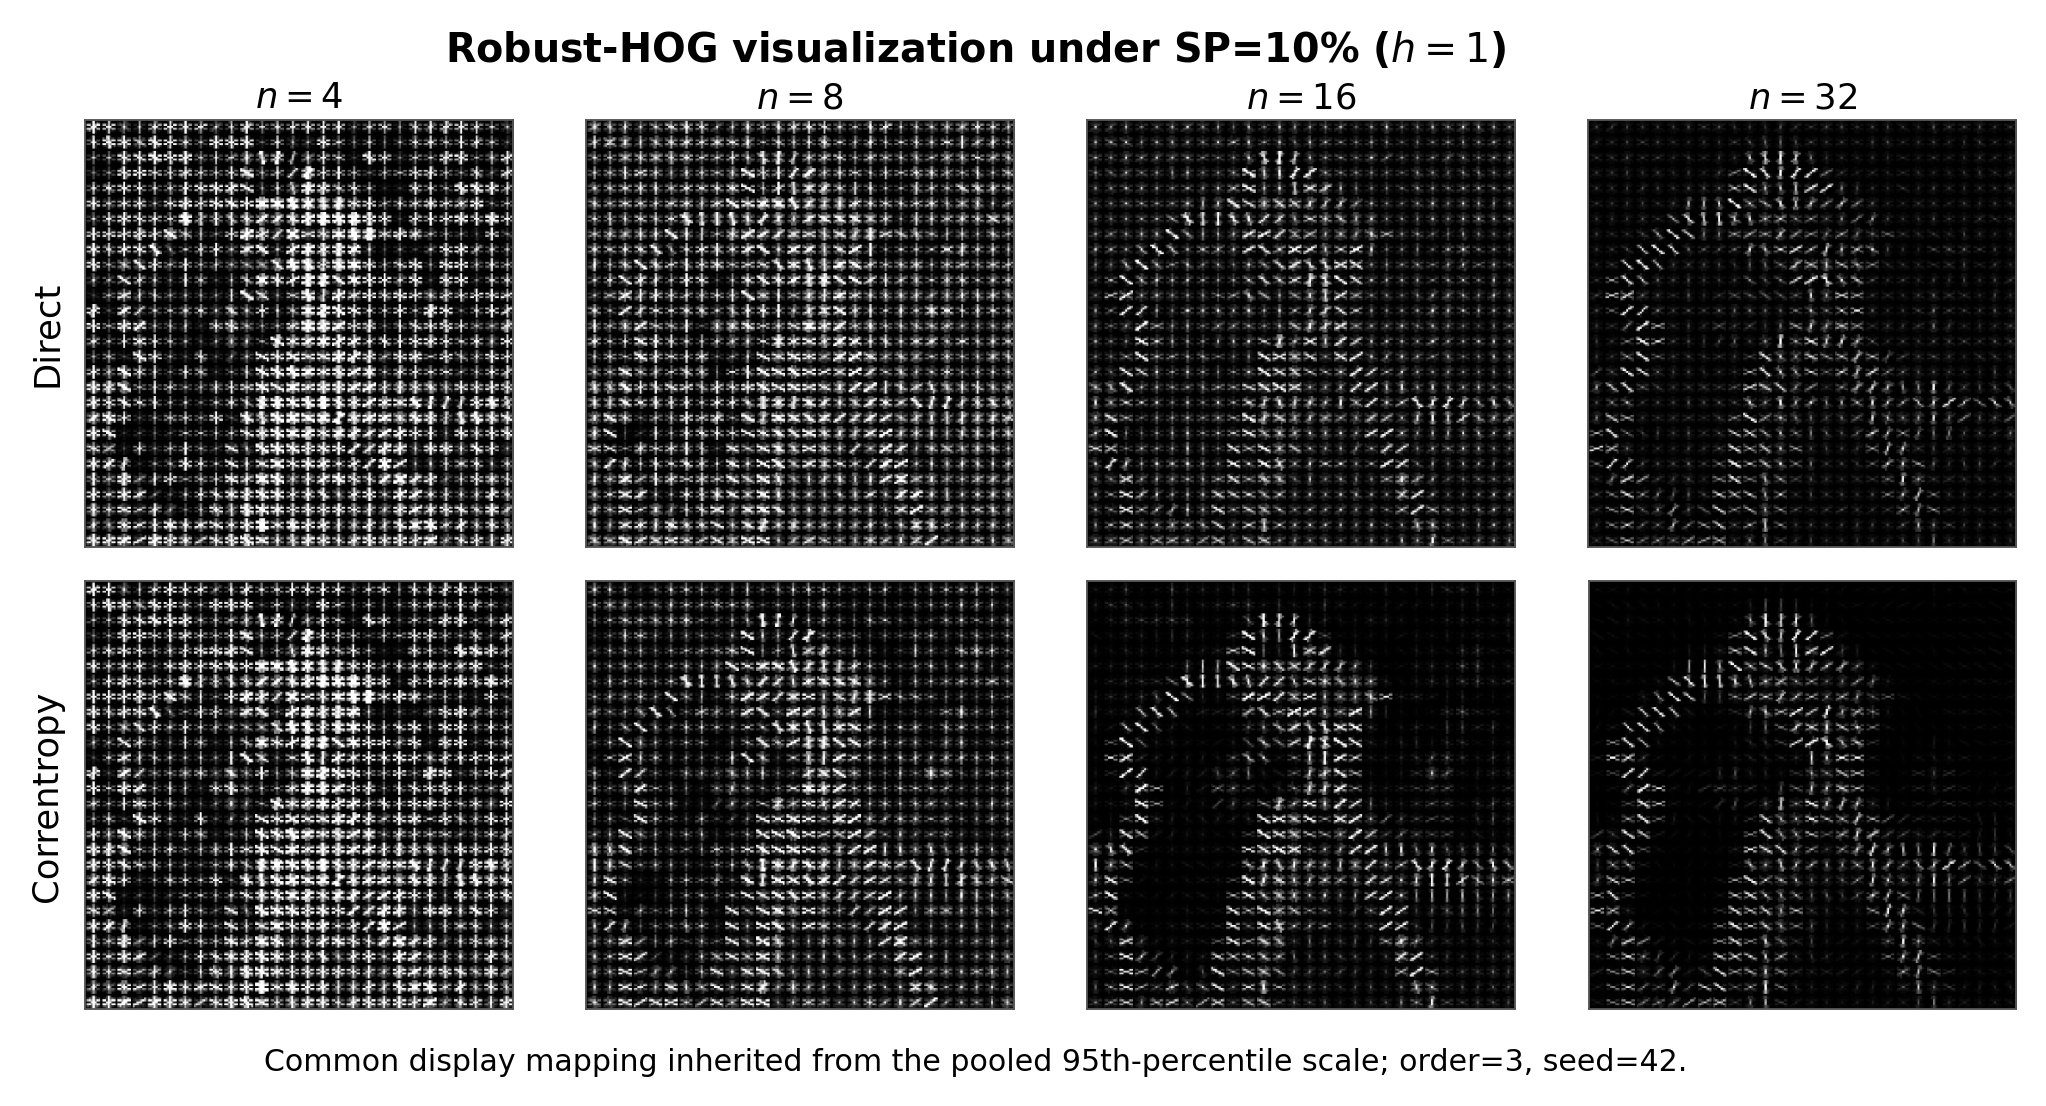
\includegraphics[width=\linewidth]{n_visual_comparison.png}
\caption{Qualitative Robust-HOG comparison for Direct and Correntropy gradients at SP 10\% while varying the per-axis sample count. All panels share the pooled 95th-percentile display scale.}
\label{fig:n-visual-comparison}
\end{figure*}

\begin{figure*}[t]
\centering
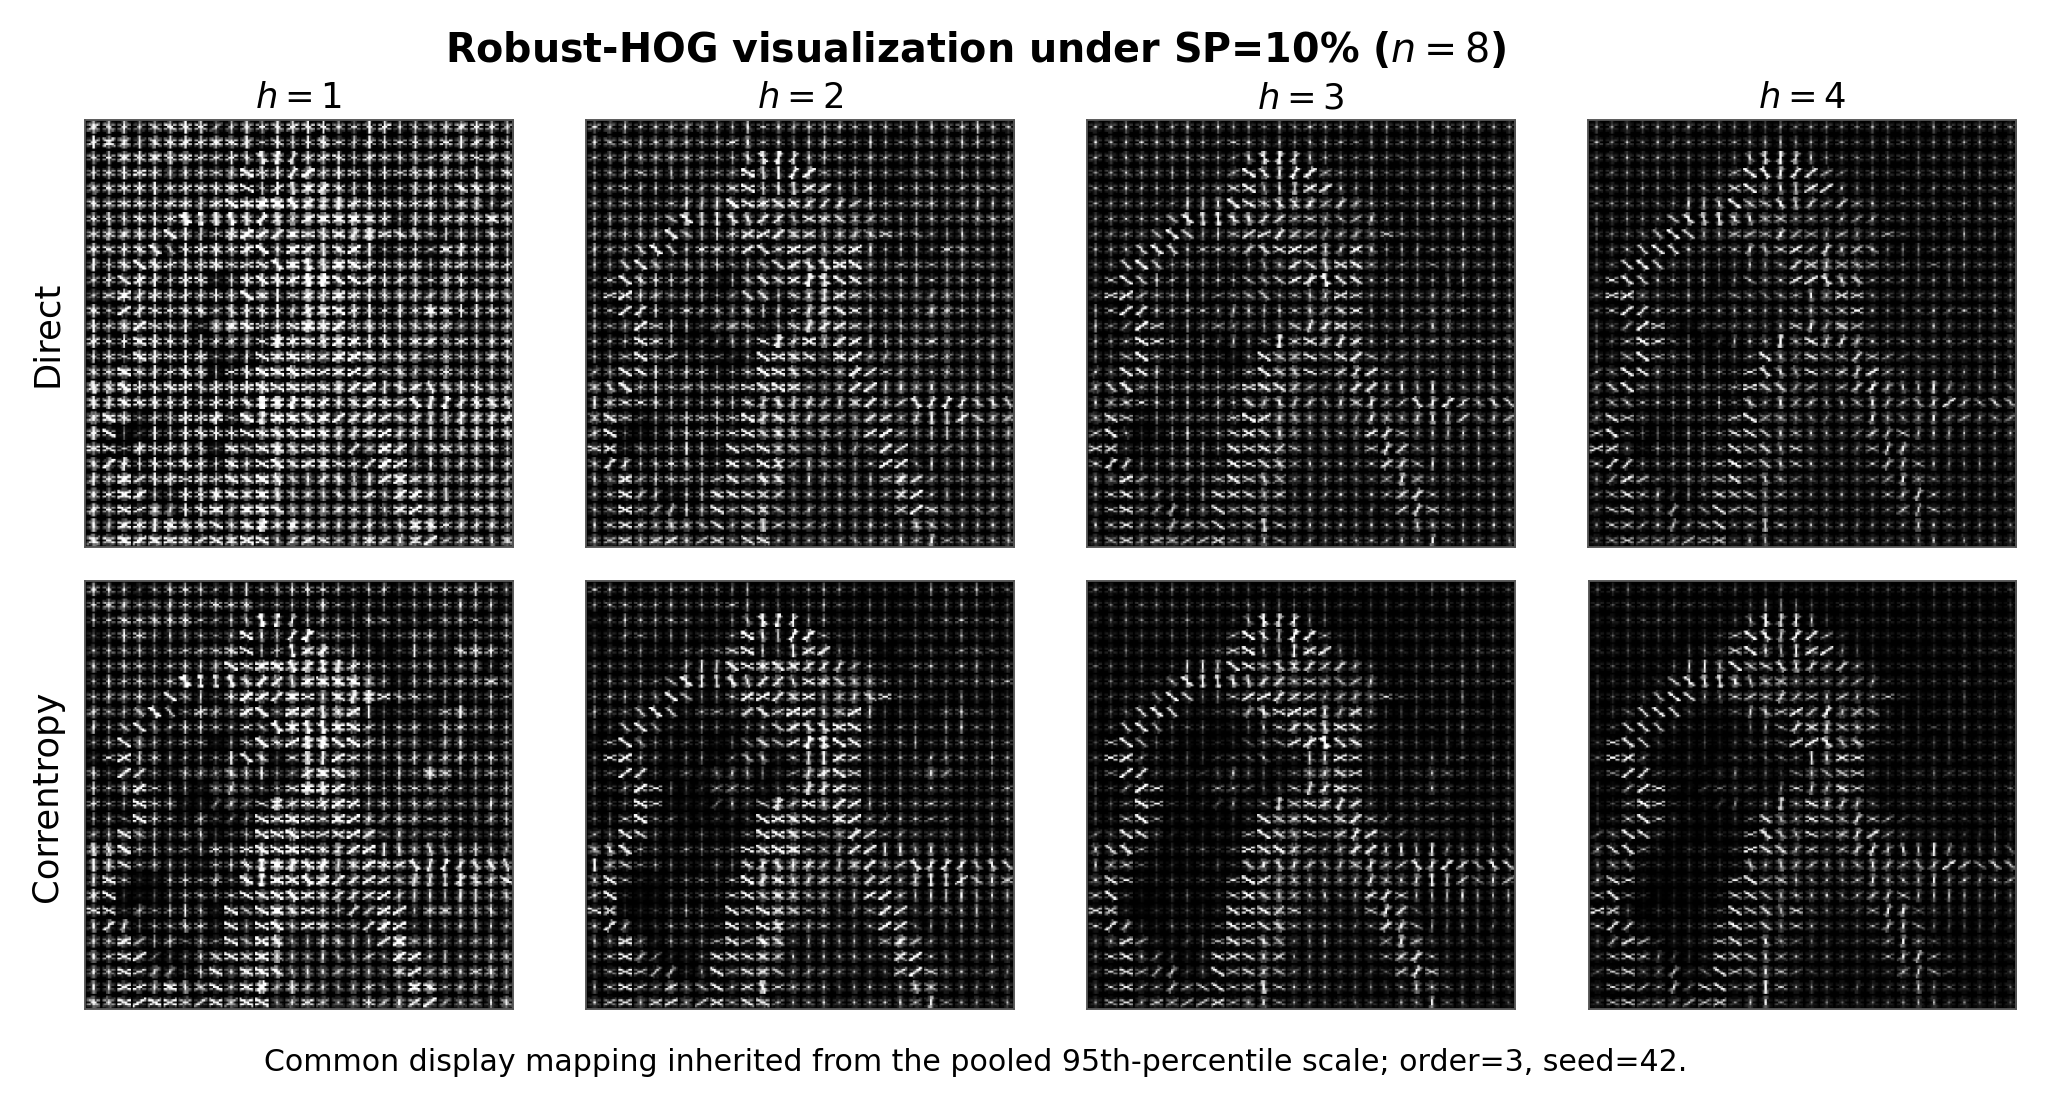
\includegraphics[width=\linewidth]{h_visual_comparison.png}
\caption{Qualitative Robust-HOG comparison for Direct and Correntropy gradients at SP 10\% while varying sample spacing. All panels share the pooled 95th-percentile display scale.}
\label{fig:h-visual-comparison}
\end{figure*}

\paragraph{Sparse joint correntropy sweep.}
The joint experiment evaluated only $(8,3)$, $(8,4)$, $(16,2)$, $(16,3)$, $(16,4)$, and $(32,1)$ under SP 5\% and SP 10\%; it is not a full factorial search. The fastest and balanced criteria both selected $(n,h)=(16,4)$, with mean runtime 10.475~s over SP 5\% and SP 10\%. The maximum-weighted-robustness selection was $(n,h)=(32,1)$, with mean runtime 25.476~s over SP 5\% and SP 10\%. Selection labels are candidate-set dependent and do not imply a universal optimum.

\IfFileExists{parameter_summary.tex}{% Generated by final_parameter_analysis.py from joint_correntropy_sweep.csv.
% Requires the booktabs package.
\begin{table*}[t]
\centering
\caption{Representative correntropy configurations from the sparse joint sweep. Matched-clean metrics quantify noise stability.}
\label{tab:parameter-summary}
\small
\setlength{\tabcolsep}{3.5pt}
\begin{tabular}{llrrrrrr}
\toprule
Role & Noise & $n$ & $h$ & RMSE & HOG rel. error & Cosine & Runtime (s) \\
\midrule
Fastest / Balanced & SP 5\% & 16 & 4 & 0.811 & 0.2338 & 0.9727 & 10.380 \\
Fastest / Balanced & SP 10\% & 16 & 4 & 1.233 & 0.3882 & 0.9246 & 10.569 \\
Maximum weighted robustness & SP 5\% & 32 & 1 & 0.977 & 0.2037 & 0.9792 & 22.813 \\
Maximum weighted robustness & SP 10\% & 32 & 1 & 1.453 & 0.3183 & 0.9493 & 28.140 \\
\bottomrule
\end{tabular}
\par\medskip
\footnotesize All rows use correntropy, polynomial order 3, seed 42, and the same 192 by 192 common analysis ROI after cropping. Fastest minimizes mean runtime. Maximum weighted robustness maximizes the normalized matched-clean quality score. Balanced maximizes the harmonic mean of that score and logarithmic runtime benefit across the six measured candidates. Raw SP 5\% and SP 10\% metrics are first averaged per configuration, then min-max normalized across the six candidates.
The fastest and balanced criteria may select the same measured configuration.
\end{table*}
}{% Generated by final_parameter_analysis.py from joint_correntropy_sweep.csv.
% Requires the booktabs package.
\begin{table*}[t]
\centering
\caption{Representative correntropy configurations from the sparse joint sweep. Matched-clean metrics quantify noise stability.}
\label{tab:parameter-summary}
\small
\setlength{\tabcolsep}{3.5pt}
\begin{tabular}{llrrrrrr}
\toprule
Role & Noise & $n$ & $h$ & RMSE & HOG rel. error & Cosine & Runtime (s) \\
\midrule
Fastest / Balanced & SP 5\% & 16 & 4 & 0.811 & 0.2338 & 0.9727 & 10.380 \\
Fastest / Balanced & SP 10\% & 16 & 4 & 1.233 & 0.3882 & 0.9246 & 10.569 \\
Maximum weighted robustness & SP 5\% & 32 & 1 & 0.977 & 0.2037 & 0.9792 & 22.813 \\
Maximum weighted robustness & SP 10\% & 32 & 1 & 1.453 & 0.3183 & 0.9493 & 28.140 \\
\bottomrule
\end{tabular}
\par\medskip
\footnotesize All rows use correntropy, polynomial order 3, seed 42, and the same 192 by 192 common analysis ROI after cropping. Fastest minimizes mean runtime. Maximum weighted robustness maximizes the normalized matched-clean quality score. Balanced maximizes the harmonic mean of that score and logarithmic runtime benefit across the six measured candidates. Raw SP 5\% and SP 10\% metrics are first averaged per configuration, then min-max normalized across the six candidates.
The fastest and balanced criteria may select the same measured configuration.
\end{table*}
}

\paragraph{Runtime scaling.}
Figure~\ref{fig:runtime-scaling} reports newly measured runtime curves rather than extrapolating from the single-size sensitivity CSV. Each panel uses the same image sizes and $n$ values, and the shared logarithmic vertical axis permits direct scale comparison. The timer includes noisy gradient estimation, common-ROI cropping, and Robust HOG, while image loading, resizing, noise generation, and design-matrix construction are excluded. For fixed $h=1$, the estimator first solves $(S-n)^2$ native gradient centres and then crops every output to the common $(S-32)^2$ ROI. The curves therefore report implementation-level pipeline runtime rather than fixed-output-pixel complexity. Correntropy timing is data and convergence dependent; monotonic runtime in $n$ is therefore not assumed. Each interquartile band is a descriptive spread over three repeats, not a confidence interval.

\begin{figure*}[t]
\centering
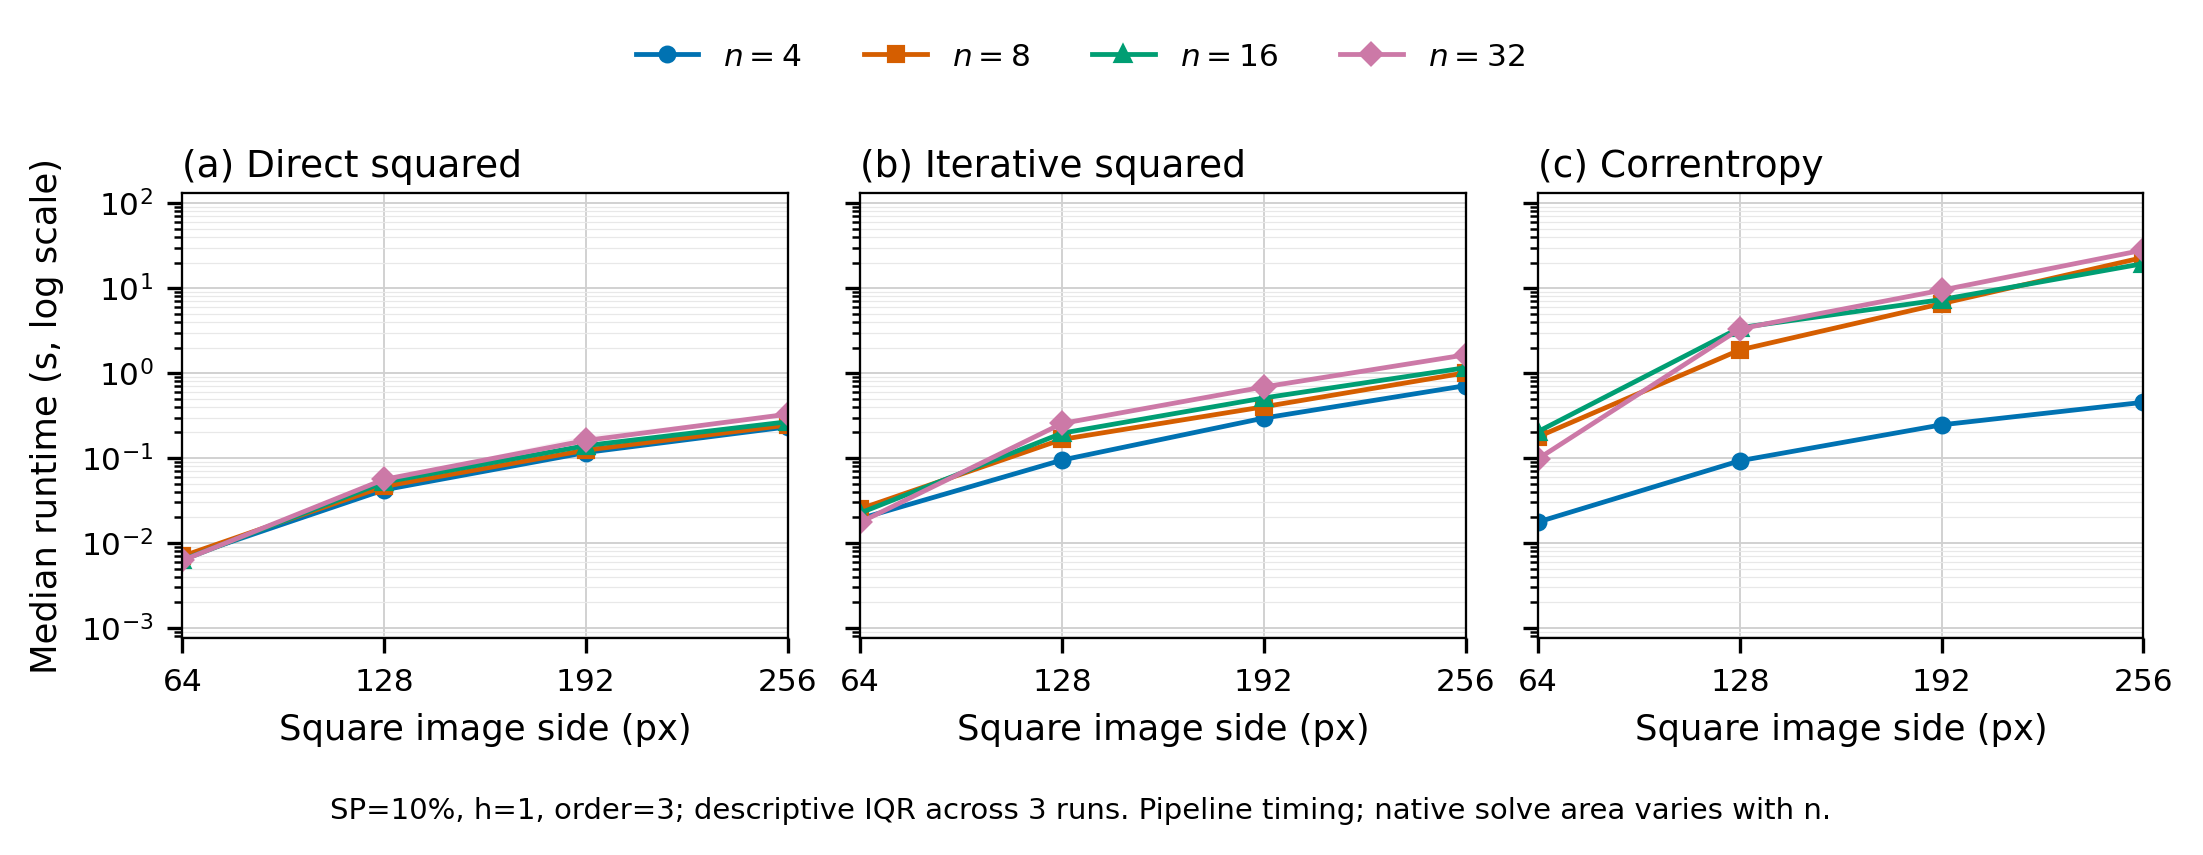
\includegraphics[width=\linewidth]{runtime_scaling_2d.png}
\caption{Median gradient-plus-HOG inference runtime versus square image side under SP 10\%, with fixed $h=1$ and order 3. Shaded bands show the descriptive interquartile range of three timing repeats; native solve area varies with $n$ before common cropping.}
\label{fig:runtime-scaling}
\end{figure*}

\paragraph{Reproducibility limitation.}
The noise realization and benchmark order use seed 42. Because only one noise seed and one source image are included, the reported values are deterministic case-study measurements rather than population estimates or confidence intervals.
